% \begin{multicols}{2}

\section{Einleitung}

\subsection{Ziel der Arbeit}

In erster Linie soll ein Computerprogramm entwickelt werden, welches aufgrund eines Höhenmodells eine möglichst defensive (risikominimierende) Aufstiegsroute plant. Als Erweiterung wird dieses Modell mit einer ansprechenden 3D-Karte als Hintergrundebene in einer öffentlich zugänglichen Web-App zur Verfügung gestellt. Die vom Modell produzierten Touren werden mit Literaturrouten aus dem Tourenportal des SAC bzw.\ aus diversen dort gesammelten Tourenführern verglichen und auf ihre Begehbarkeit kritisch überprüft.

\subsection{Bestehende Referenzsysteme}

Mit dem Algorithmus von Andreas Eisenhut besteht seit 2013 eine mehr oder weniger fertig implementierte Lösung um Skitouren im Gelände automatisch zu planen\ \cite{eisenhuttourknopfdruck}. Trotz der starken Abhängigkeit von kostenpflichtigen Werkzeugen stellt diese Arbeit eine Pionierleistung in diesem Gebiet dar und wurde ebenfalls durch die Plattform Skitourenguru aufgegriffen. Hier ist es jedoch nutzerseitig nicht möglich, eine Navigation von einem Start- zu einem Zielpunkt durchzuführen. Zum Verfassungszeitpunkt dieser Arbeit kann die öffentlich zugängliche Version des Tools nur verwendet werden, um bestehende GPS-Tracks und von Hand gezeichnete Routen idealer zu legen. Die Thesis von A. Eisenhut wurde während des Implementationsprozesses dieser Arbeit nicht referenziert, erst während des Verfassens der finalen Arbeit.

\subsection{Begriffe und Definitionen}

Diverse Akronyme werden im Anhang/Abkürzungsverzeichnis definiert. Es empfiehlt sich, diesen Abschnitt im Voraus zu konsultieren. Weitere Begriffserklärungen sind in den Fusszeilen zu finden.

\clearpage
\section{Grundlagen der Lawinenkunde}
\subsection{Ziel der Lawinenkunde}

Konkret steht eine Entscheidung im Vordergrund: <<GO / NO-GO>>. Ist mit den aktuell vorherrschenden Wetterbedingungen eine Tour mit akzeptierbarem Restrisiko möglich? Welche Vorsichtsmassnahmen müssen dazu getroffen werden? Gibt es Schlüsselstellen, welche nicht durchquert werden dürfen? In der modernen Lawinenkunde wird der Fokus vor allem auf die Praxis gelegt. <<Wie kann das bestehende Risiko eingeschätzt werden?>> Während früher vor allem ein Fokus auf Bergungsmethoden gelegt wurde, wird heute vermehrt präventiv gearbeitet.~\cite{harveyrhynerschweizerlawinenkunde}

Ein Literaturklassiker im Bereich der Lawinenkunde ist beispielsweise Werner Munters \citetitle{munter}, in welchem erstmals nebst dem Gelände und den Verhältnissen auch der Faktor <<Mensch>> betrachtet wurde~\cite{munter}. In dieser Arbeit wird der Schwerpunkt auf den Faktor <<Gelände>> gelegt.

\subsection{Lawinentypen}

Lawinen lassen sich klassifizieren anhand ihrer Auslösemechanismen, des Materials, welches sie transportieren, und der spezifischen Bedingungen, unter denen sie entstehen. Die wichtigsten Lawinentypen -- Schneebrettlawinen, Lockerschneelawinen, Gleitschneelawinen (und Staublawinen) -- unterscheiden sich in ihrer Entstehung, Dynamik und den daraus resultierenden Gefahren~\cite{harveyrhynerschweizerlawinenkunde}. Eine genaue Kenntnis dieser Unterschiede ist für die Lawinenkunde und das alpine Risikomanagement notwendig. In Abb. \ref{fig:lawinentypen} sind die wichtigsten Lawinentypen grafisch dargestellt (+ 4. Staublawinen, welche vermehrt im Himalaya auftreten)~\cite{ortovoxlabsnow}.
\skiplines{2}
\begin{figure}[H]
  \centering
  \includegraphics[width=\linewidth]{UeberischtLawinen_mark}
  \caption{Wichtigsten Lawinentypen~\cite{ortovoxlabsnow}}\label{fig:lawinentypen}
\end{figure}
\pagebreak
\begin{enumerate}
  \item Schneebrettlawinen~\cite{harveyrhynerschweizerlawinenkunde}\cite{sacbergspwinter}\cite{slfLawinentypen}\cite{ortovoxlabsnow}:
  \begin{itemize}
    \item Fordern 90\% der Lawinenopfer
    \item 98\% aller Lawinentoten sterben in Schneebrettlawinen
    \item Abriss entlang einer Kante, Schnee gleitet als ganzer Block, als <<Brett>> ab
    \item Brett gleitet auf einer darunterliegenden Schwachschicht in der Schneedecke ab
    \item Kann aufgrund von Mehrbelastung durch Wintersportler oder spontan abgehen
    \item Auslösender Athlet steht oft mitten im Schneebrett
    \item Verschüttungsgefahr: gross – Mitreiss- \& Absturzgefahr: gross
    \item Gefahr ab einer Hangneigung von $30\degree$
  \end{itemize}
  % % \columnbreak{}
    
  \item Lockerschneelawinen~\cite{harveyrhynerschweizerlawinenkunde}\cite{sacbergspwinter}\cite{slfLawinentypen}:
  \begin{itemize}
    \item Punktförmiger Auslösepunkt
    \item Reisst immer mehr Schnee mit; kegelförmiger Abgang, der nach unten breiter wird
    \item Verschüttungsgefahr: klein – Mitreiss- \& Absturzgefahr: gross
    \item Im Auslösepunkt ist meistens eine hohe Steigung von $40\degree$ notwendig
  \end{itemize}

  \item Gleitschneelawinen~\cite{harveyrhynerschweizerlawinenkunde}\cite{sacbergspwinter}\cite{slfLawinentypen}:
  \begin{itemize}
    \item Linienförmige Abrisskante
    \item Die gesamte Schneedecke gleitet ab
    \item Geringe Bedeutung für Wintersportler –-- gehen oft spontan ab und gefährden vor allem Infrastruktur (Abgleiten erfolgt über mehrere Stunden oder Tage hinweg, zeigt sich gut durch sog. <<Fischmäuler>>)
  \end{itemize}
\end{enumerate}
Für unsere Zwecke interessieren uns an erster Stelle \textbf{Schneebrettlawinen} und an zweiter \textbf{Lockerschneelawinen}, da diese Lawinentypen abseits der Schweizer Pisten für die meisten Unfälle mit Personenschaden  verantwortlich sind~\cite{harveyrhynerschweizerlawinenkunde}.
In $\qty{95}{\percent}$ aller Unfälle lösen Schneesportler dabei ihre Unglückslawine selbst aus~\cite{ortovoxlabsnow}. Aus diesem Grund wird im weiteren Verlauf dieser Arbeit einer möglichen Fernauslösung keine weitere Beachtung geschenkt. Damit wird vor allem verhindert, dass flächendeckend auf Basis von zu langen oder falsch eingeschätzten Ablagerungsbereichen ein zu hohes Risiko vorhergesagt wird.~\cite{athmaps}

\pagebreak
\subsection{Typische Lawinenprobleme}\label{lawinenprobleme}

In der Lawinenkunde werden bestimmte Lawinenprobleme definiert, um die komplexen Zusammenhänge einfacher verständlich zu machen und die Risikoanalyse zu erleichtern. Diese typischen Lawinenprobleme umfassen verschiedene Szenarien, die besonders häufig auftreten und die Lawinengefahr massgeblich beeinflussen. Ein tiefes Verständnis dieser Probleme ist erforderlich, um im gefährdetem Gelände sicher unterwegs zu sein und präzise Entscheidungen in Bezug auf Lawinensicherheit zu treffen. Es werden vier Lawinenprobleme unterschieden:

\begin{enumerate}
  \item Neuschneeproblem~\cite{harveyrhynerschweizerlawinenkunde}\cite{achtunglawine}:
  \begin{itemize}
    \item Frischer Neuschnee, welcher sich schlecht mit den darunterliegenden Schneeschichten verbunden hat
    \item Produziert ab der kritischen Neuschneemenge (je nach Bedingungen zwischen \qty{10}{cm} und \qty{50}{cm}) mindestens die Warnstufe <<3 -~Erheblich>> im \acrfull{llb}
    \item Setzt sich innerhalb von zwei bis drei Tagen
  \end{itemize}
  \item Triebschneeproblem~\cite{harveyrhynerschweizerlawinenkunde}\cite{achtunglawine}:
  \begin{itemize}
    \item Wind trägt Neuschnee in Windschattenlagen
    \item Triebschnee verbindet sich leicht mit sich selbst, jedoch nicht mit darunterliegenden Schichten; ideale Voraussetzungen für ein Schneebrett
    \item Gefahr durch Schneeverfrachtungen (z.B. Wechten)
    \item Setzt sich innert zwei bis drei Tagen
  \end{itemize}
  \item Nassschneeproblem~\cite{harveyrhynerschweizerlawinenkunde}\cite{achtunglawine}:
  \begin{itemize}
    \item Die Schneedecke wird durch eindringendes Wasser geschwächt
    \item Die erste Durchfeuchtung führt zu der bedeutendsten Schwächung
    \item Gefahr nach andauernden Regenperioden im Winter
    \item Typische Frühlingslawinen, steigende Gefahr im Verlauf des Tages mit steigender Temperatur
    \item Lang anhaltende Gefahr
  \end{itemize}
  \item Altschneeproblem~\cite{harveyrhynerschweizerlawinenkunde}\cite{achtunglawine}:
  \begin{itemize}
    \item z.B. eingeschneite Harschschichten schwächen die Schneedecke erheblich
    \item Dauert Wochen bis Monate an
  \end{itemize}
\end{enumerate}
Es ist möglich, dass mehrere Lawinenprobleme kombiniert auftreten. Im \gls{llb} sind jeweils alle zu erwartenden Lawinenprobleme mit einer eigenen Gefahrenstufe aufgeführt.~\cite{slfTypischeLawinenprobleme}

\subsection{Lawinenlagebericht (Bulletin) \& Gefahrenstufen}

Im Lawinenbulletin/Lawinenlagebericht (\gls{llb}), werden die momentan am Berg zu erwartenden Lawinenprobleme (siehe~\ref{lawinenprobleme}) zusammengefasst und mit diversen zusätzlichen Daten ergänzt~\cite{lawinengefskala}.
Abb.\ \ref{fig:bulletin} zeigt ein Beispiel eines \gls{llb} Bulletins, wie dieses während des Winters täglich erscheint.
In der europäischen Lawinengefahrenskala werden fünf Warnstufen unterschieden, von <<1 -~gering>> bis <<5 -~sehr gross>>~\cite{harveyrhynerschweizerlawinenkunde}\cite{lawinengefskala}.
Rund 50\% der Unfälle geschehen dabei bei Stufe <<3~-~mässig>>.~\cite{achtunglawine}
\begin{figure}[H]
  \centering
  \includegraphics[width=7.5cm]{bulletin}
  \caption{Bulletin vom 12.2.24~\cite{slfarchiv}}\label{fig:bulletin}
\end{figure}
Die Skala ist kontinuierlich, jedoch nicht linear. Dies bedeutet konkret: 
Im Durchschnitt ist das Risiko bei <<mässig>> fünfmal grösser als bei <<gering>>, und bei <<erheblich>> dreimal grösser als bei <<mässig>>~\cite{sacbergspwinter} (siehe Abb.\ \ref{fig:llbdanger}).
\begin{figure}[H]
  \centering
  \includegraphics[width=7cm]{gefahrenstufen}
  \caption{Die 5 europäsischen Lawinengefahrstufen in einem Graph}\label{fig:llbdanger}
\end{figure}
Um die Einteilung dieser fünf Kategorien weiter zu verfeinern, wurden in der Schweiz zusätzlich Teilabstufen durch $+$, $-$ und $=$ eingeführt (So lautet die Warnstufe im Bericht nun z.B.\ $3+$, wenn die tatsächliche Gefahr bereits nahe an einer $4$ bzw.\ $4-$ liegt).~\cite{sacbergspwinter}
Unterschiedliche Interpretationen der standartisierten europäischen Skala sorgen leider dafür, dass Differenzen zwischen schweizerischen und ausländischen Vorhersagen bestehen. Dies stellt besonders in Grenzregionen ein Problem dar. Nachfolgend wird dies jedoch nicht weiter thematisiert.

\pagebreak
\subsection{Lawinenbildende Faktoren}

Lawinen sind das Resultat eines unglücklichen Zusammenspiels dreier wesentlicher Faktoren: 
\textbf{Verhältnisse} (Wetterlage und Zustand der Schneedecke), \textbf{Gelände} (Neigung, Exposition, Höhe) und \textbf{Mensch} (95\% aller Lawinen mit Personenschaden wurden durch Menschen ausgelöst)~\cite{ortovoxlabsnow}.

Weder die Verhältnisse noch das Gelände lassen sich direkt von Wintersportlern beeinflussen. Nur durch die Wahl eines anderen Datums (nur in Ausnahmefällen sinnvoll, z.B.\ bei einer Expedition), oder durch eine geschickte Spuranlage lassen sich diese Faktoren mildern. 
Ist beides keine Option, muss eine alternative Tour ausgewählt werden.
Den bei weitem grössten Einfluss hat die maximale Hangneigung -- daher konzentrieren sich die meisten gängigen Reduktionsmethoden wie die \gls{grm} und der Avulator\footnote{Gängiger Entscheidungsrahmen in Kanada} vor allem darauf~\cite{arpddatasetdocs}\cite{harveyrhynerschweizerlawinenkunde}.

\subsection{Munters 3~\texttimes~3 Schema}
Der Goldstandard der heutigen Tourenplanung ist Werner Munters $3\times3$-Schema. Dabei werden in drei <<Zoom>>-Stufen drei Faktoren ausgewertet:
% \vfill


\begin{table}[hb] 
  \centering
  \renewcommand{\arraystretch}{2}
  \begin{tabular}{|p{0.13\linewidth} | p{0.25\linewidth} | p{0.25\linewidth} | p{0.27\linewidth} |}
    \hhline{|----|}
   &  \textbf{Verhältnisse} & \textbf{Gelände} & \textbf{Mensch} \\
   \hhline{|----|}
  \textbf{Regional} &  1.~Lawinenlagebericht \par 2.~Wetterprognose \par 3.~Auskünfte von Einheimischen/ Hüttenwart &  1.~Karte $1:25000$ \par 2.~Tourenführer \par 3.~Eigene Geländekentnisse & 1.~Wer ist dabei? \par 2.~Ausbildung \par 3.~Material \par 4.~Mentale und physische Kondition?  \\ \hhline{|----|}
  \textbf{Lokal} & 1.~Sicht? \par 2.~Bewölkung, Wind, Niederschlag, Temperatur? \par 3.~Schneeverfrachtungen, Neuschneemenge \par 4.~Stimmt der \gls{llb}? & 1.~Stimmt meine Vorstellung (Steilheit, Exposition)? \par 2.~Spuren anderer Gruppen & 1.~Ausrüstungskontrolle (Gruppencheck \acrshort{lvs}, Harscheisen dabei?) \par 2.~Andere Gruppen unterwegs? \\ \hhline{|----|}
  \textbf{Zonal} & 1.~Neuschneemenge \par 2.~Triebschnee \par 3.~Mögliche Abrisszonen \par 4.~Sonneneinstrahlung & 1.~Wer / was ist über/unter der Gruppe? \par 2.~Steilste Stelle? \par 3.~Exposition,\par 4.~Typisches Lawinengelände \par 5.~Hangform \par 6.~Höhe \par 7.~Oft befahren? & 1.~Können und Kondition \par 2.~Vorischtsmassnahmen \par 3.~Sichere Sammelstellen \\
   \hhline{|----|}
  \end{tabular}
  \renewcommand{\arraystretch}{1}
  \caption{Das Schema 3$\times$3~\cite{munter}}\label{tab:3x3table}
\end{table}

\pagebreak
\subsection{Grafische Reduktionsmethode \& relevante Geländefaktoren}

Die momentan am meisten verwendete Reduktionsmethode ist die sogenannte grafische Reduktionsmethode.\ Bei dieser wird -- je nach prognostizierter Ausprägung eines Lawinenproblems -- nur die lokale Hangneigung zur Entscheidungsfindung eingesetzt~\cite{sacbergspwinter}. In der Planungsphase wird die Hangneigung aus einer $1:25000$er-Karte mittels Neigungsmesser herausgelesen. Dies liefert jedoch nur die durchschnittliche Neigung des Geländes zwischen den Höhenlinien -- einen möglichen steileren Hangabschnitt sieht man also nicht.
Unterwegs kann entweder unter Zuhilfenahme von Smartphone, Skistöcken oder Pendel die Hangneigung ermittelt werden. Es kann nun in der Grafik (siehe Abb.\ \ref{fig:grm}) herausgelesen werden, ob das zu überprüfende Gelände problemlos, nur mit Vorsichtsmassnahmen wie Entlastungsabständen oder gar nicht betreten werden darf.
%TODO: Anhang mit Hangneigungsbestimmung Stocks
\begin{figure}[H]
  \centering
  \includegraphics[width=\linewidth]{grm}
  \caption{\gls{grm}-Karte~\cite{achtunglawine}}\label{fig:grm}
\end{figure}

Der starke Fokus auf die Hangneigung ist ein häufiger Kritikpunkt an der grafischen Reduktionsmethode. Deshalb wird diese oft zusammen mit sogenannten <<Mustern>> gelehrt. Diese beschreiben bestimmte Warnzeichen und wie diese das Risiko beeinflussen~\cite{achtunglawine}. Dabei wird beispielsweise auf <<Fischmäuler>> geachtet, welche ein Gleitschneeproblem im Hang anzeigen~\cite{harveyrhynerschweizerlawinenkunde}. Letztendlich bleibt die \gls{grm} jedoch, wie der Name verrät, eine Reduktionsmethode -- es werden selektiv die in die Auswertung einfliessenden Parameter reduziert.

\subsection{Unfalldaten \& Begehungen}

Hänge, deren steilste Stelle mindestens 30° geneigt ist gelten als lawinengefährdet. Etwa 19° geneigtes Gelände wird am häufigsten begangen, bis 40° steigt das Lawinenrisiko enorm an und bleibt danach hoch. Auf eine eigene Auswertung von Unfalldaten wird in dieser Arbeit verzichtet, hier hat der \acrfull{sac} zusammen mit der Skitourenguru GmbH bereits wertvolle Vorarbeit geleistet. So konnten die berechneten Risikoverteilungen direkt übernommen werden.~\cite{sacbergspwinterp99} 


\clearpage
\section{Geoinformatische Grundlagen}

\subsection{Digitale Höhenmodelle}\label{sec:dem}

In den 1960er Jahren verlangte der Schweizer Generalstab vom heutigen Bundesamt für Landestopografie zu prüfen, ob tief fliegende feindliche Kampfflugzeuge unbemerkt in den Schweizer Luftraum eindringen könnten. Um die für dieses Vorhaben nötigen Berechnungen erstmals an einem Grossrechner ausführen zu können, mussten die topografischen Höhen aus der Landeskarte $1:25000$ auf Lochkarten transferiert werden. Mit einer Auflösung von \qty{250}{m} wurden die Höhenlinien der analogen Kartenprodukte so in mühseliger Handarbeit zwischen 1966 --~1968 erstmals digital nutzbar gemacht. Das so erstellte digitale Höhenmodell (\acrshort{dem} / \acrshort{dhm}) <<RIMINI>> wurde bis in die 1970er Jahre genutzt.~\cite{swisstopohistdem}

Rufe nach einem engmaschigeren Modell brachten schliesslich unter anderem das <<DHM25>> hervor, welches Daten in einer Auflösung von bereits \qty{25}{m} mitbrachte.~\cite{swisstopohistdem}

Um die Jahrtausendwende erfolgte dank schnelleren Rechenkernen und günstigerem Datenspeicher eine Umkehrung des Prozesses. Neu werden die analogen Landeskarten auf Grund eines \acrshort{dem} erstellt. Moderne DEMs erreichen dabei eine Auflösung bis zu \qty{0.5}{m} bei einer Genauigkeit von 0.5 --~3 \unit{m} und werden direkt aus Lasermessungen oder stereokorrelierten Luftbildern abgeleitet~\cite{alti3dprod}. SwissAlti\textsuperscript{3D} ist genau solches ein Modell.

Dank der <<Open Government Data Strategie>> des Bundes werden seit 2020 diverse Datensammlungen die öffentliche Verwaltungen produzieren der Öffentlichkeit wieder zur Verfügung gestellt~\cite{opendataswiss}.
So landet nebst dem Fahrplan der SBB, Jungwaldflächen und den Standorten aller öffentlichen Toiletten der Stadt Luzern (und unzähligen weiteren Datensätzen) auch  SwissAlti\textsuperscript{3D} auf dem Open Data Portal des Bundes (\url{https://opendata.swiss/}).
Dieses wird als GeoTIFF ausgeliefert. GeoTIFF sind verlustfrei komprimierte Bilddaten, welche um einen Eintrag zur Lokalisierung in einem Koordinatensystem, hier LV95 LN02, ergänzt wurden. Der Farbwert eines Pixel entspricht jeweils der Höhe an dieser Stelle. Insgesamt wird die Schweiz in ca. $43500$ $\qty{1}{km} \times \qty{1}{km}$ grosse Kacheln unterteilt.~\cite{alti3dprod} 

Aus einem solchen Höhenmodell lässt sich die Hangneigung viel präziser und hochauflösender herauslesen, als dies von Hand aus einer $1:25000$er-Karte möglich ist.

\subsection{Digitale Landschaftsmodelle}

Berge, Wälder, Flüsse und Seen sind ebenfalls ein wichtiger Kartenbestandteil. Auf Skitour gilt es zum Beispiel Schwimmpassagen zu vermeiden. Swisstopo liefert mit SwissTLM\textsuperscript{3D} einen Datensatz, welcher alle auf einer Landeskarte ersichtlichen Objekte enthält. Im weiteren Verlauf interessieren uns hier vor allem stehende und fliessende Gewässer, gewässerüberquerende Brücken, sowie Wald- und Wildruhezonen.

\subsection{Geoinformationssysteme (GIS)}\label{sec:gis}

\acrshort{gis} sind leistungsstarke Werkzeuge, die zur Analyse, Darstellung und Interpretation von geografischen Daten verwendet werden. Mit einem solchen Werkzeug können etwa geografische Karten verfasst, ökologische Veränderungen überwacht oder zoologische Migrationsmuster analysiert werden.
In dieser Arbeit wurde das quelloffene Werkzeug QGIS extensiv verwendet; zudem wurde eine eigene Analyse-Erweiterung entwickelt~\cite{qgis}. QGIS wurde gegenüber anderen kommerziellen \acrshort{gis}-Lösungen gewählt, da diese oft teuer verrechnet werden.

\subsection{Einführung in die Graphentheorie}

Ein Graph beschreibt wie eine Menge von Knotenpunkten (Verticies) $V$ durch die Kanten (Edges) $E$ verbunden sind. Ein Graph kann gerichtet oder ungerichtet sein: Ein gerichteter Graph beschreibt eine Beziehung zwischen zwei Knoten, wobei diese Beziehung nur in eine Richtung verläuft. Ein ungerichteter Graph beschreibt eine Beziehung, welche in beide Richtungen verläuft. Ein Graph kann zudem gewichtet sein, wobei die Kanten mit einem Wert bzw. Kosten versehen sind. Ein gewichteter Graph wird oft zur Modellierung von Netzwerken verwendet, beispielsweise können Schienen- oder Strassennetzwerke so modelliert werden. In diesem Fall entsprechen die Knoten den Haltestellen bzw. Kreuzungen, die Kanten den Verbindungen zwischen diesen und die Kosten den Fahrzeiten oder Distanzen.
Da in dieser Arbeit mit einem diskreten Gitter gearbeitet wird, wird ein ungerichteter, gewichteter Graph verwendet. Die Knoten entsprechen den Gitterpunkten, die Kanten den möglichen Bewegungen zwischen den Punkten und die Gewichte den Kosten der Bewegung. Wir verbinden alle Gitterzellen mit ihren acht Nachbarn, analog zu allen Zügen, die für den König auf einem Schachbrett möglich sind.


\subsection{Algorithmus von Dijkstra und A*}

Die Suche nach einem Pfad mit minimalen Kosten lässt sich formal als Graphen-Problem darstellen und lösen. Dabei wird jeder Gitterpunkt zu einem Knotenpunkt in einem Graph, welcher durch acht ungerichteter Kanten mit seinen Nachbarn verbunden ist. So kann das Problem bereits mit dem Algorithmus von Dijkstra gelöst werden.~\cite{dijkstra1959note}

Es wird eine leere Vorrangwarteschlange\footnote{Eine Liste von Elementen, die bereits beim Einfügen anhand eines Wertes sortiert werden.} initialisiert, welcher sofort der dem Ursprungspunkt entsprechenden Knoten mit Kosten 0 hinzugefügt wird. Die laufenden Kosten aller anderen Knoten werden auf $+ \infty$ gesetzt. Es werden nun fortlaufend folgende zwei Schritte ausgeführt, bis der Knoten, welcher der Zielzelle entspricht, erweitert wurde.~\cite{dijkstra1959note}
\begin{itemize}
  \item \textbf{Selektion:} Es wird fortgefahren mit jenem Knoten, der die geringsten laufenden Kosten hat. Zu Beginn entspricht dies dem Startknoten mit Kosten 0. Dank der Vorrangwarteschlange ist dies trivial möglich, da diese Datenstruktur ein Element bereits beim dessen Einfügen am richtigen Ort einsortieren kann. Mit dem Abrufen des vordersten Elements aus der Warteschlange, wird dieses auch entfernt.~\cite{dijkstra1959note}
  \item \textbf{Erweitern:} Es wird durch die Nachbarn des aktuellen Knotens iteriert. Jeden Nachbarn, bei dem die Summe aus den laufenden Kosten des aktuellen Knotens, den Gitterkosten des Nachbarn sowie den Bewegungskosten zwischen den beiden Zellen geringer ist, als dessen bisherige Kosten, wird mit der oben errechneten Summe als Priorität der Warteschlange hinzugefügt (und die laufenden Kosten des Knotens überschrieben). Formal sind die zu minimierenden Kosten hier $f(n)=g(n)$, wobei $n$ dem nächsten Knoten und $g(n)$ den laufenden Kosten vom Start zum Knoten $n$ entspricht. Ausserdem wird gespeichert, von welcher Zelle aus die Nachbarn jeweils erreicht wurden.~\cite{dijkstra1959note}
\end{itemize}

Da jeweils der Vorgänger von jeder Zelle gespeichert wurde, kann am Ende der Pfad vom Ende zum Start hin zurückverfolgt werden. So können nicht nur die gesamten Kosten, sondern auch der rekonstruierte Pfad als Lösung erhalten~\cite{dijkstra1959note}.

Eine implementierte Erweiterung die auf dem Algorithmus von Dijkstra aufbaut, wird als A* (A-Star) bezeichnet. Hier wird die Berechnung der zu minimierenden Kosten um eine Heuristik $h(n)$ (eine Schätzung der verbleibenden Kosten) erweitert. Formal werden die zu minimierenden Kosten neu also $f(n)=g(n)+h(n)$.~\cite{Hart1968}

Als Heuristik wird im weiteren Verlauf der Arbeit die Taxi- bzw. Chebyshev-Distanz verwendet~\cite{cantrell2000modern}. Der Beweis für die Zulässigkeit der Heuristik wird dem Leser als Übung überlassen. 

\subsection{Naismith'sche Regel}

Nebst den risikoabhängigen Durchgangskosten, werden auch Bewegungskosten berücksichtigt. Diese beschreiben die Zeit und Anstrengung die benötigt wird, um einen Meter Weg zurückzulegen. Eine weitverbreitete und akzeptierte Schätzungsmethode ist die sogenannte Naismith'sche Regel~\cite{naismithsrule}.
Beim Skitouren wird dabei je \qty{4000}{m} Horizontaldistanz und je \qty{400}{hm} Vertikaldistanz eine Stunde Wegzeit gerechnet~\cite{sacbergspwinter}\cite{naismithsrule}. 
Zum Beispiel wird für eine \qty{6000}{m} lange Tour mit \qty{800}{hm} Anstieg wird eine Aufstiegsdauer von $\frac{\qty{6000}{m}}{\qty{4000}{m\per\hour}} + \frac{\qty{800}{hm}}{\qty{400}{hm\per\hour}} = \qty{3}{h}\ \qty{30}{\min}$ angenommen.

\subsection{Berechnung topografischer Oberflächenfaktoren}
Ziel ist die Berechnung der charakteristischen Geländeeigenschaften für die Zelle $e$.
Von Interesse sind Aspekt, Neigung und Krümmung.
Dazu wird ein $3 \times 3$-Ausschnitt aus dem Höhenmodell betrachtet. 
$a$~--~$h$ sind die Höhen der Gitterpunkte rund um unserer Zielzelle \textbf{e}:

\begin{figure}[H]
  \centering
  \includegraphics[width=7.5cm]{isoGrid}
  \caption{$3 \times 3$-Ausschnitt von Höhen aus einem \acrshort{dem} und deren Benennung}
\end{figure}

In der Praxis wurden diese Berechnungen mit dem Werkzeug \code{gdaldem} ausgeführt, nach dem ein eigenes Programm keinen erheblichen Leistungsvorteil erzielt hatte. Die detaillierten Formeln zur Berechnung aller Eigenschaften finden sich im Anhang~\ref{app:formeln}.


\vfill

\pagebreak


\section{Methodik}

Zu Beginn der Arbeit war ein Ziel, möglichst unabhängig von Software-Bibliotheken und fremdem Code zu bleiben. Während der Machbarkeitsstudie wurde jedoch festgestellt, dass es letztlich sinnvoll ist, auf eine kommerzielle \acrshort{gis}-Lösung~(siehe~\ref{sec:gis}) zu setzten -- analog zur \acrshort{unix}-Philosophie~\cite{unixphil}. Diese gilt als Orientierungshilfe, wie Software entworfen werden soll. Unter anderem soll zum Beispiel jeweils die simpelste, funktionale Lösung gewählt werden, Software modular aufgebaut sein und nur einen Zweck erfüllen~\cite{unixphil}. Tausende Stunden Entwicklungsarbeit stecken bereits in \acrshort{gdal} (\acrlong{gdal}) und QGIS, auf welchen gerne aufgebaut wurde~\cite{gdalmanual}\cite{qgis}.
\subsection{Herunterladen des Höhenmodells}

Wie bereits in Kap.\ \ref{sec:dem} erwähnt, wird SwissAlti\textsuperscript{3D} in $\qty{1}{km} \times \qty{1}{km}$ grossen Kacheln ausgeliefert, welche einzeln heruntergeladen und anschliessend wieder vereint werden müssen~\cite{alti3dprod}. Auf dem Datenportal von swisstopo kann für jeden Kanton eine Liste mit den URLs der Kacheln, welche in dem Kanton liegen, heruntergeladen werden. Mittels eines Python-Skriptes wurden so über Nacht knapp \qty{30}{GB} Höhendaten der Kantone BE, GL, GR, NW, OW, SZ, UR und VS heruntergeladen. Durch \code{gdal\_warp}, \code{rasterio} und \code{gdal2tiles}\footnote{Diverse GIS-Werkzeuge} wird als Erstes eine Kopie in einem für die Webkarte lesbaren Datenformat erstellt. Statt Höhenwerte direkt aus dem Pixelraster zu lesen, werden diese auf die drei RGB-Farbkanäle verteilt. So schlüsselt der rote Farbwert nun einzelne Höhenmeter, der blaue Kanal 256 hm und der grüne $256^2$ hm auf. Beispiele beider Encodierungsmethoden sind in Abb.\ \ref{fig:dem} zu sehen.

\begin{figure}[H]
  \centering
  \includegraphics[width=\linewidth]{dem}
  \caption{Höhenmodell der Schweizer Alpenkantone in je einem RGBDEM-Tileset und einem schwarz-weissen GeoTIFF. Die dunklen Flecken links sind Höhen über 3100 m. ü. M.}\label{fig:dem}
\end{figure}

\subsection{Erstellung von Risikokarten}

Als Grundlage für alle weiteren Schritte werden Risikokarten benötigt; ursprünglich hätten tatsächliche Lawinenabgänge simuliert werden sollen. In RAMMS::Avalanche\footnote{Lawinensimulationsprogramm entwickelt am SLF} wurden zuerst Initialisierungspolygone, also Flächen, welche durch Schneesportler ausgelöst werden könnten, gesucht und dann mittels einer Standardlawinensituation (50cm Neuschnee, Lockerschneeproblematik) ausgelöst und simuliert. Dies stellte sich aufgrund der hohen Rechenanforderungen und der damit verbunden Budget- \& Zeitanforderungen als nicht praktikabel heraus.

Stattdessen soll nur die Hangneigung $\rho$ betrachtet werden, da diese Geländeeigenschaft den höchsten Korrelationsfaktor mit der Anzahl von Lawinenereignissen bildet~\cite{arpddatasetdocs}. Dies ist in der \gls{grm} bereits gebräuchlich. Auf die Analyse der Geländekrümmung wird verzichtet, da diese auf die tatsächliche Route praktisch keinen Einfluss hat.\\
Der Risikowert einer einzelnen Zelle wird gemäss~\citeauthor{sacbergspwinterp99}~\cite{sacbergspwinterp99} folgendermassen berechnet:

\[
r(\rho) = \sqrt{\frac{1}{1 + e^{\frac{s-\rho}{3.0}}}}
\]

Je nach prognostizierter Gefahrenstufe des \gls{llb} wird $s$ zwischen 20 und 35 linear interpoliert. Im Fall der Gefahrenstufe 3= kommt $s$ dabei bei 28.0 zu liegen. (siehe Abb.~\ref{fig:graph} für die resultierende Risikofunktion)

Mittels eines Python-Skripts und des Pakets \code{rasterio} wurde diese Berechnung am gesamten Gitter ausgeführt.

\begin{figure}[H]
  \centering
  \includegraphics[width=6.5cm]{graph_cellfriction}
  \caption{Graph der modellierten Risikofunktion $r(\rho)$ für $0 \leq \rho \leq 90$ \\bei prognostizierter Gefahrenstufe 3=}\label{fig:graph}
\end{figure}

\subsection{Parallele Berechnungen}

Um die Berechnung der Risikokarte effizient zu gestalten und alle auf dem Rechner verfügbaren Ressourcen zu verwenden, wird die Berechnung in kleinen Kacheln ausgeführt, welche dann zusammengepuzzelt werden. Die einzelnen Kacheln werden dabei auf der \acrshort{gpu} verarbeitet. Letztlich ist diese Berechnung ein grafisches Problem, welches durch die Grafikeinheit mit ihren vielen parallel arbeitenden Rechenkernen um ein Vielfaches schneller gelöst werden kann.

\subsection{Wasserquerungen und Brücken}

SwissTLM\textsuperscript{3D} liefert den Verlauf von Strassen und Gewässern. Zuerst werden die Daten so gefiltert, dass nur noch Oberflächengewässer und Strassenabschnitte, die als Brücke deklariert sind im Datensatz vorhanden sind.

In QGIS werden nun alle Gewässerflächen um einen Radius von \qty{7.5}{m} <<gepuffert>>, also erweitert. Die resultierenden Gewässerpolygone werden gerastert und mit einem Risikowert von $9 \times 10^{9}$ in die rohe Risikokarte eingebrannt. Anschliessend wird dasselbe mit den Brücken wiederholt; hier wird jedoch das Risiko auf $0.0$ gesetzt. Somit sind Gewässer für den Algorithmus ein absolutes Tabu und werden nur bei Brücken überquert. Auf das Abwägen ob eine Überquerung möglich ist, wurde aus praktischen Gründen verzichtet. In solchen Fällen kann eine Tour anhand der rohen Risikokarte geplant werden.

\pagebreak
\subsection{QGIS-Plugin LeastCostWalk}

Um den Algorithmus von Dijkstra nun auch auszuführen, musste eine neue Erweiterung für QGIS in Python implementiert werden. Ein Auszug des Quellcodes befindet sich im Anhang. Gegenüber bestehenden Least-Cost-Plugins verfügt meine Implementierung über die Funktionalität, Wegzeit/Bewegungskosten gegen Reibungs- bzw. Risikokosten abzuwägen. Dies geschieht anhand 5 Parametern 

\begin{itemize}
  \item $k_{risk}$, wie schwer die Risikokosten ins Gewicht fallen,
  \item $c_{steepascend}$ / $c_{steepdescend}$, wie stark steile Auf- \& Abstiegspassagen gewichtet werden,
  \item $c_{flat}$, wie teuer Horizontaldistanz ist,
  \item $c_{ascend}$ / $c_{descend}$, wie teuer ein normaler Auf- \& Abstieg ist.
\end{itemize}
Die jeweiligen Quantitäten werden mit ihren Koeffizienten gewichtet und summiert.

Nebst den Kostenkoeffizienten werden Start- \& Zielpunkt, die Koordinatenreferenzsysteme dieser Punkte, das Höhenmodell und die Risikokarte an das Modell übergeben. Wird die Erweiterung in der grafischen Oberfläche von QGIS gestartet, entspricht dies Abb.\ \ref{fig:qgisplugin}. Das gesamte Modell ist in der Abb.\ \ref{fig:walkmodel} ersichtlich. Wird das Modell als Endanwendung genutzt, wird vor dem Start der tatsächlichen Berechnungen das Gebiet der Tour aus der Risikokarte und dem \acrshort{dhm} ausgeschnitten. So können die benötigten Rechenressourcen eingegrenzt werden.

Im Fall der Webanwendung wird die Erweiterung serverseitig über die Kommandozeile (\acrshort{cli}) automatisch aufgerufen.

\begin{figure}[H]
  \centering
  \includegraphics[width=7.5cm]{qgisplugin}
  \caption{QGIS-Erweiterung <<LeastCostWalk>> in der grafischen Oberfläche von QGIS}\label{fig:qgisplugin}
\end{figure}

\subsection{Server Deployment mit Docker}

Um ein einfaches Bereitstellen zu ermöglichen und auf diese Weise die horizontale Skalierbarkeit\footnote{Statt einen einzelnen Server mit mehr bzw.\ leistungsstärkerer Hardware zu bestücken, kann ein weiterer zugeschaltet bzw. <<horizontal>> daneben gestellt werden.} der Server-Ressource zu gewährleisten, wurde ein Docker-Image\footnote{Vereinfacht gesagt: Ein Miniaturbetriebssystem, das innert Sekunden auf diversen Rechnern als Gastsystem hochgefahren werden kann und vom Rest des Systems isoliert ist.} erstellt. Darin wurde die \gls{gis}-Anwendung sowie die Risikokarten und das Höhenmodell vorinstalliert. Momentan läuft die Anwendung auf einem Miniaturserver unter Ubuntu Server 24.04 LTS.\ Der Vorteil der hier gewählten Paketierung ist jedoch, dass auch andere Serverbetriebssysteme ohne Änderung des eigentlichen Quellcodes unterstützt werden (inklusive Windows, Ubuntu, Debian und FreeBSD). Zusätzliche Instanzen könnten ebenfalls zugeschaltet werden, um eine durchgehend verfügbare öffentliche Version für 100 --~1000 Nutzer pro Stunde ohne lange Wartezeiten zur Verfügung zu stellen.

% \clearpage
\subsection{3D-Karte im Webbrowser}

Als Erweiterung zum reinen \gls{gis}-Modell wurde eine Webanwendung in Vue.js und MapLibre GL JS realisiert~\cite{vuedevman}\cite{maplibregljs}. Als Basislayer für die Karte wurde das Layer <<Vector Base Map>> von swisstopo verwendet, welches durch die Höhendaten von SwissAlti\textsuperscript{3D} in eine dreidimensionale Form gebracht wurde~\cite{basevtprod}\cite{alti3dprod}. Nutzer können sich mittels eines Google-Accounts anmelden und ihre Routen so persönlich abspeichern und wieder aufrufen. Zusätzlich steht basierend auf den in SwissTLM verfügbaren Lokalnamen eine Suchfunktion zur Verfügung.
Die Planung einer neuen Tour kann durch die Auswahl von Start- \& Zielort sowie der gewünschten Modellvariante in Auftrag gegeben werden -- innert ca.\ \qty{20}{s} ist das Resultat verfügbar und wird dem Nutzer direkt angezeigt.

% \end{multicols}

% \begin{Mappage}
  \begin{figure}[H]
    \centering
    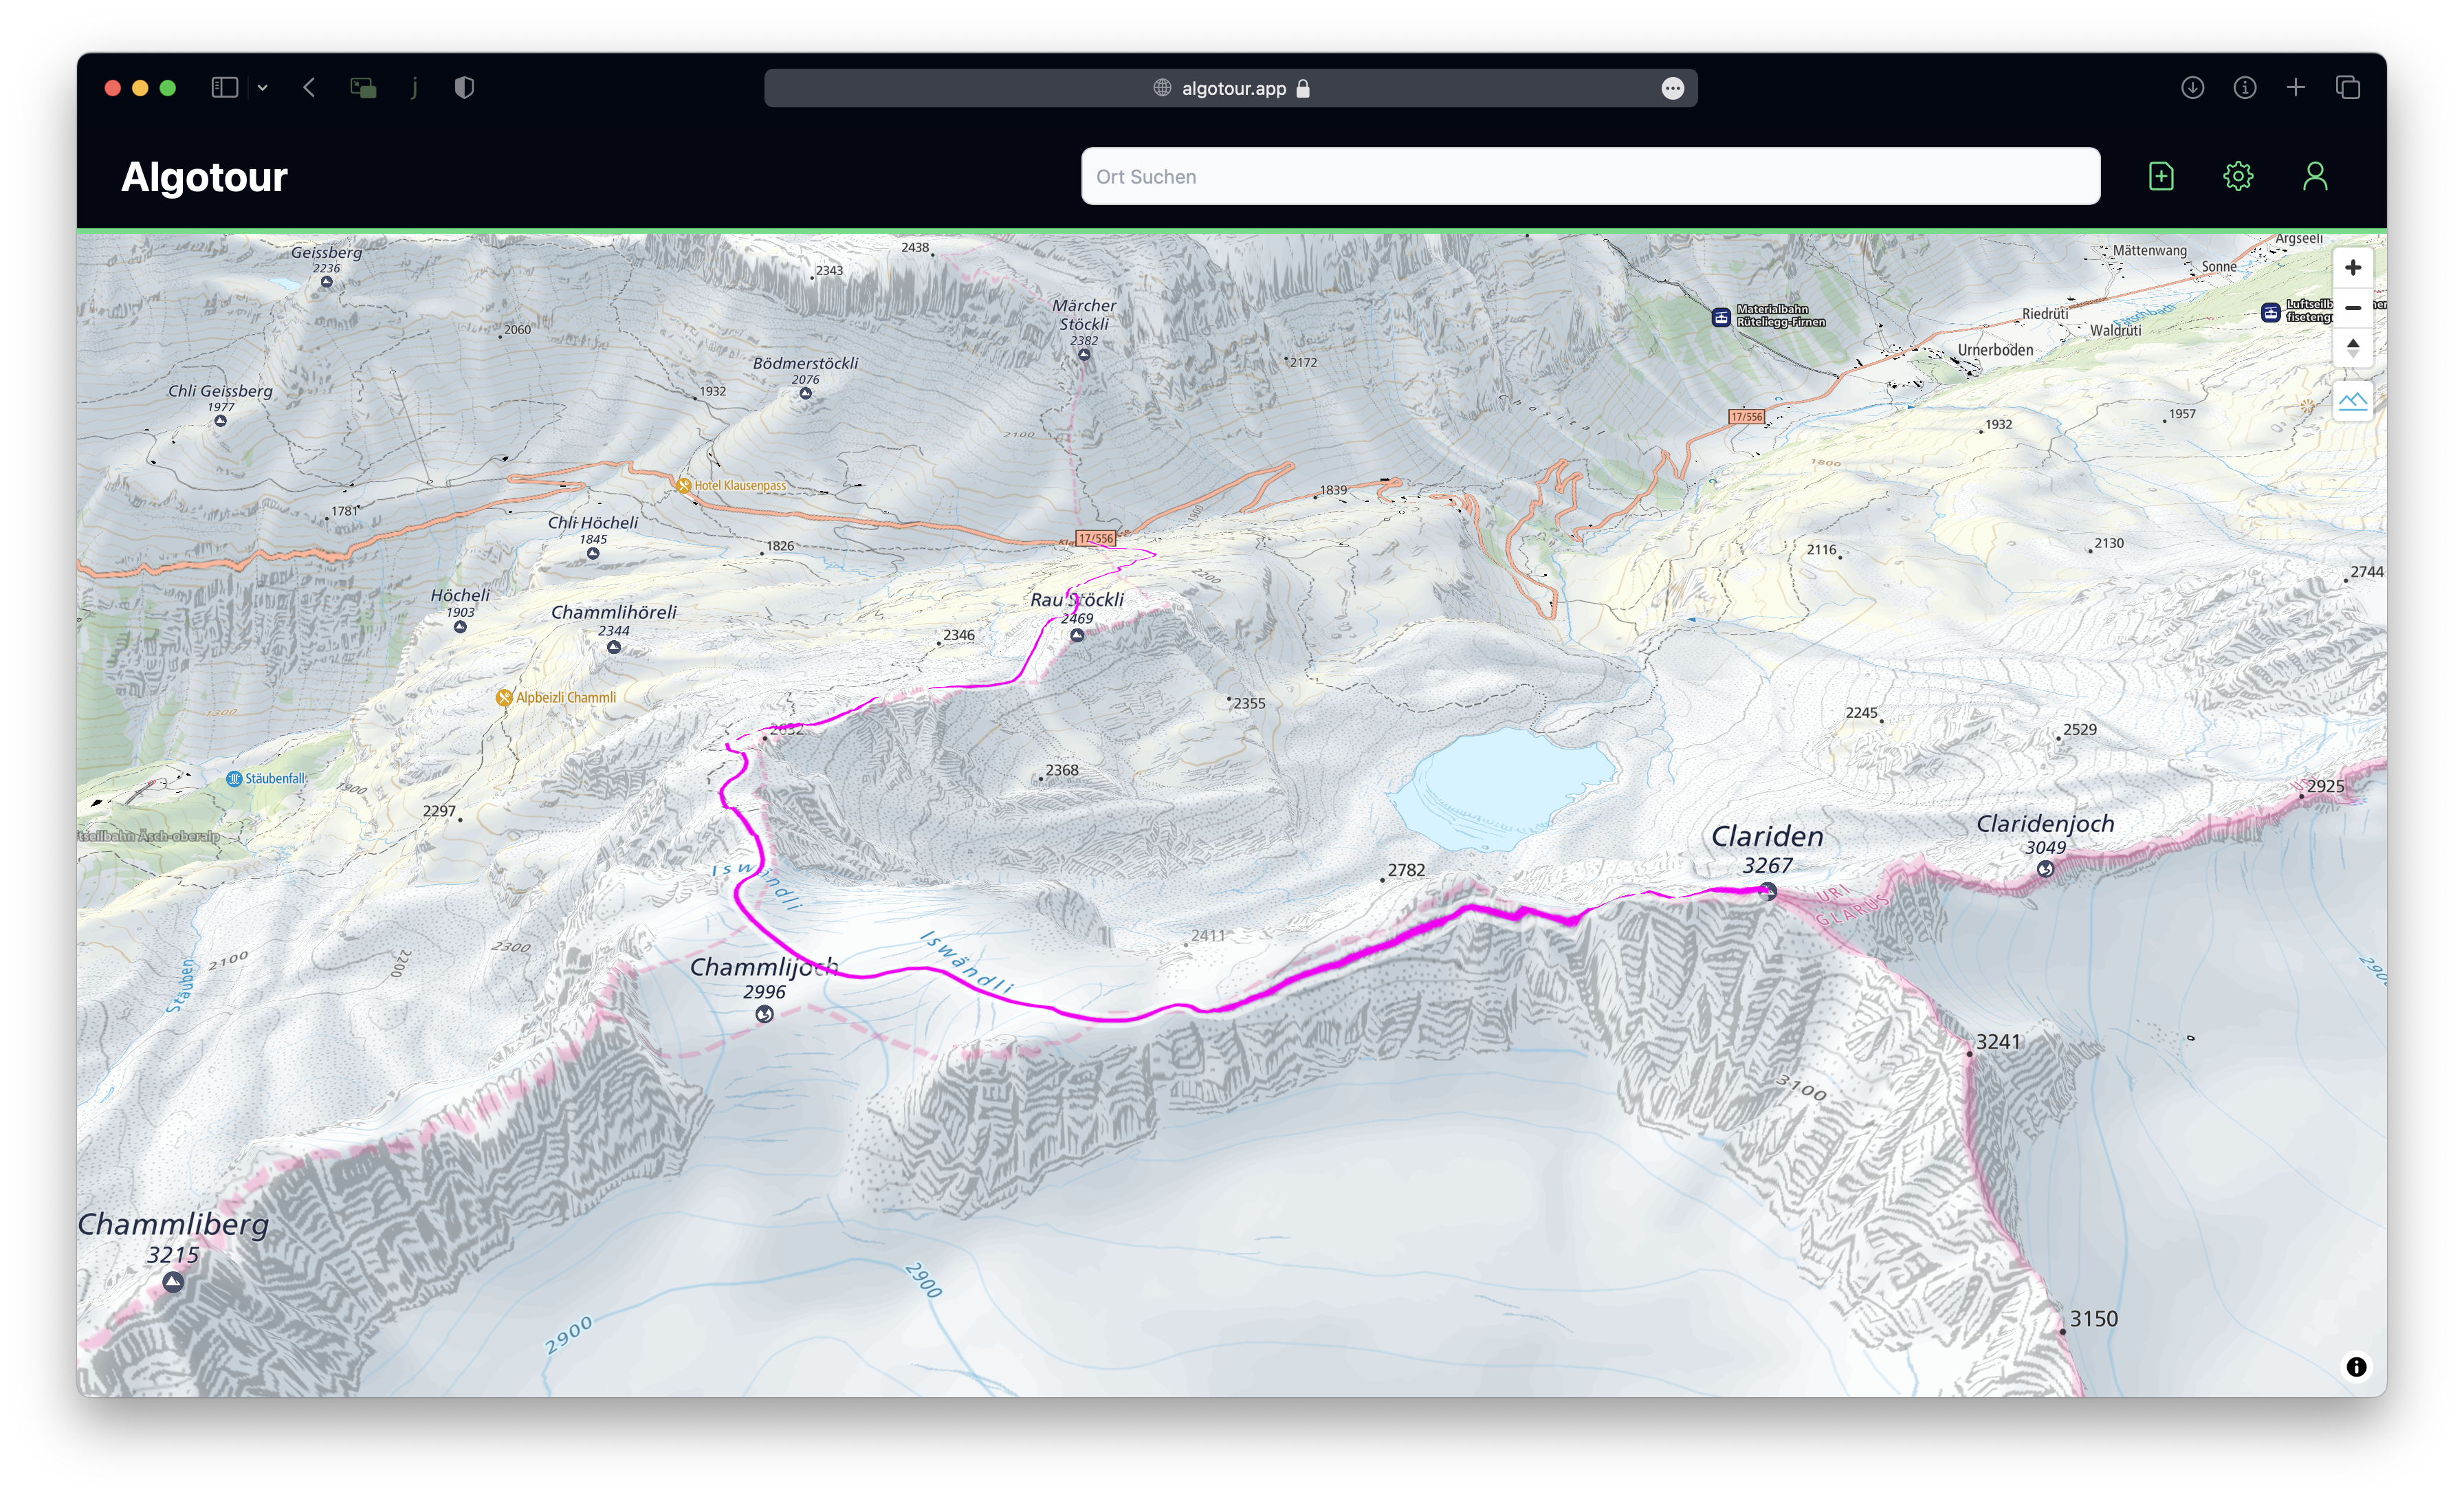
\includegraphics[width=\linewidth]{webapp}
    \caption{Nutzeroberfläche der Web-App, Tour auf den Clariden}\label{fig:mainui}
  \end{figure}
  % \end{Mappage}

% \begin{multicols}{2}


% \end{multicols}
